\documentclass[12pt, letterpaper]{article}
%packages
\usepackage[english]{babel}
\usepackage[utf8]{inputenc}
\usepackage{fancyhdr}%headers/footers
\usepackage{hyperref}%hyper links
\usepackage{amsmath}%fractions and such
\usepackage{listings}%code listing
\usepackage{graphicx}%iamges
\usepackage{float}% H placement parameter - less floaty floats

%document metadata
\title{First document}
\author{Rastislav Kučera}
\date{June 2018}

%page style defines
\fancypagestyle{MyDefault}{\pagestyle{fancy}\fancyhf{}\cfoot{\thepage}}

\fancypagestyle{MyFirstPage}{\pagestyle{fancy}\fancyhf{}\rhead{Rastislav Kučera}\lhead{Ročníkový projekt (2)}}

%newcommand


%document setup
\pagestyle{MyDefault}
\hypersetup{
    colorlinks=true,
    linkcolor=blue,
    filecolor=magenta,      
    urlcolor=cyan,
}
\graphicspath{ {./images/} }%image directory


\begin{document}

\begin{titlepage}\centering
\thispagestyle{MyFirstPage}
%Centering and title
\vspace*{\fill}
\LARGE \textbf{General representation of light sources in photorealistic computer graphics} 
\vspace*{\fill}
\end{titlepage}

\section{Introduction}
This project models various light sources 
%later also materials and geometry
and describes their generalization for rendering based on \href{http://www.cse.chalmers.se/edu/year/2011/course/TDA361/2007/rend_eq.pdf}{rendering equation} using \href{https://en.wikipedia.org/wiki/Monte_Carlo_method}{Monte Carlo method}.
The rendering equation can be expressed as \\
%add nice indentation ... later
$I(x,x') = g(x,x')[e(x,x') + \int_{S}^{} p(x,x',x'')I(x',x'')dx$] , where:\\ 
$I(x,x')$ is related to the intensity of light passing from point $x'$ to point $x$\\
$g(x,x')$ is "geometry" term \\
$e(x,x')$ is related to the intensity of emitted light from $x'$ to $x$\\
$p(x,x',x'')$ is related to the intensity of light scattered from $x''$ to $x$ by a patch of surface at $x'$\\

%mybe add something about reccurent nature of Rendering equation and how it reflects on rendering proces ...







\section{Light Source}
%Emissive Case 
Direct approach to solve The rendering equation require that light sources act as "light intensity in direction generators". Sampling of such light source will result in \textbf{Beams} - structures containing \textbf{SpatialData} or $x$ and $x'$ and \textbf{ColorData} or intensity of emitted light (with some color - wavelength), what is special case of $I(x,x')$.Because sampling can be done indefinitely, ColorData cannot contain definitive value. That has to be interpolated using data from all other Beams and intensity of light source. Light source has to emit all of its power, which means that sum of all beams intensities is equal to the intensity of Light source they originate from. Knowing this, we can set all Beam intensity to (SourcePower)/(NumberOfBeams)
%$\dfrac{SourcePower}{NumberOfBeams}$ %this is too tall for line
and rely on extensive enough sampling of Light source, which  will generate different colors with different weights. Thus every Light source should implement methods \verb|Beam getNextBeam()| - which returns some Beam, and \verb|long getNumberOfBeams()| - which returns how many Beams were created by this light Source. Beams have to contain SpatialData, ColorData and reference for their parent light source. Light Sources can be then add to renderer which supports their Beam type by serialization.
%maybe add fun fuct : beams are more Rendering equation element, LS are more MonteCarlo element

%add small comments to Reflective And Transmissive case - involves materials
\underline{Therefore, every Light Sources must implement this interface:}
\begin{lstlisting}[language=Java]
interface LightSource extends java.io.Serializable{
	Beam getNextBeam();
	long getNumberOfBeams();
}
\end{lstlisting}

\underline{Beam is abstract class that generally looks like this:}
\begin{lstlisting}[language=Java]
public Beam{
	public SpatialData sd;
	public LightSource parent;
	public ColorData c;
}
\end{lstlisting}

%the 3. function is Beam getDeterministicBeam(PointToIntersect, wavelength) which returns beam that goes somewhere from parent LS, througth Point PointToIntersect with wavelength or nothing. (maybe modifie beam power value) 

\subsection{Beam color representation}
Human eyes have 3 cones (S,M,L) which perceive color. They are sensitive to different, overlapping parts of visible light spectrum, and are more sensitive to different wavelengths in their corresponding part of light spectrum. This means that color does not depend only on which wavelengths are hitting your eye, but also on how many fotons with same/different wave length are there.

Based on this is \textbf{RGB color model}, which represent color as RGB triplet (r,g,b) - how much of each of the red, green, and blue is included. Because of that, its impossible to reconstruct full spectrum of light from RGB, which is needed for realistic representation of light effects like \href{https://en.wikipedia.org/wiki/Refraction}{refraction of light}, \href{https://en.wikipedia.org/wiki/Fluorescence}{fluorescence}, color perception of objects illuminated with differently colored lights (Apparent color), and probably more. Instead of RGB, I will use in this text Spectral representation of color, using Spectral Power Distribution so aforementioned effects would be more realistic.

\subsubsection{Spectral power distribution}
\textbf{Spectral power distribution} or SPD for short, represents how much energy is radiated on each wavelength. It can be directly used as wavelength weight in weighted random generation. \textbf{SPD should have integral equal to 1}, so its easy to scale their power on Light source.

\underline{All SPDs have to implement this interface}:
\begin{lstlisting}[language=Java]
interface SpectralPowerDistribution{
	double getNextLambda();
	double getValue(double lambda);
	double[] getFirstAndLastLambda();
}
\end{lstlisting}
where \verb|double getNextLambda()| is for wavelength sampling and \verb|double getValue(double lambda)| returns value of lambda on normalized SPD. 

\begin{figure}[H]%need to find/create normalized SPD picture
\centering 
%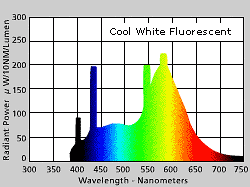
\includegraphics[natwidth=250,natwidth=187]{Spd.png}
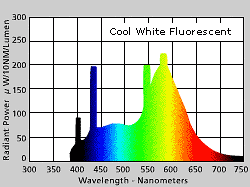
\includegraphics{Spd.png}
\caption{SPD example from \href{http://www.lrc.rpi.edu/education/learning/terminology/spectralpowerdistribution.asp}{this website}}
\end{figure}

\subsection{Sampling}
This sections describes how to take discrete samples and turn them into weighted random generators. Such process is needed for Beams SpatialData and ColorData generation. 

Discrete samples - finite number of outputs with their counts. 

Weighted random generator - return 1 output between lowest discreet sample and highest. After finite calls to this generator, resulting output distribution would be similar to the original sample distribution.
\begin{figure}[H]
\centering 
%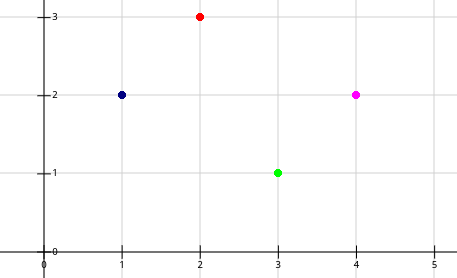
\includegraphics[natwidth=457,natwidth=278]{Samples.png}
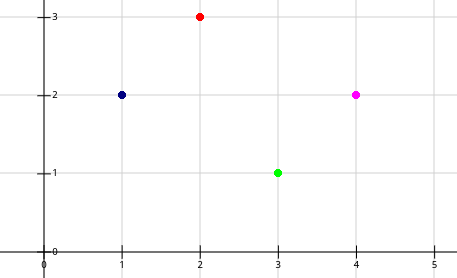
\includegraphics[scale=0.8]{Samples.png}
\caption{discrete samples}
\end{figure}

X is what we want to get, Y is the weight of desired X.

That means that we want same amount of 1s as 4s, but only half as many 3s as 1s (or 4s) and three times more 2s than 3s. 
An easy solution is to compute the sum of functional values  form 1 to 4 of this sample, which is 8, and then produce random number m form [0,1) , multiply it with found sum and then  sum  functional values until our sum is greater than m*8. Our random number from this weighted distribution is the last X used in sum. \textit{I use sum instead of integral, because we do not care about step size in this case.}

\underline{Generalization:} 
We have samples on uniformly spaced set \{a,...,b\}  with values of f(x), x belongs to \{a,...,b\}
\begin{enumerate}
\item Calculate $I = \sum_{n=a}^{b}f(n)$
\item Calculate $i = m*I$, m is random number from $[0,1)$
\item Find greatest $r$ from $\sum_{n=a}^{r}f(n) < i$, where $r$ is result
\end{enumerate}

Problem with this solution is that it creates “Choppy” distribution,what can be suppressed by adding more samples (what would reduce “choppynes”, but increase number of iterations), but not in all  cases, or by replacing gaps with some function that is easy to integrate which would remove “choppynes” completely and make this generator continuous, in which case we have to solve $\int_{a}^{r}h(x) = m*\int_{a}^{b}g(x)$, where $r$ is the result and $h(x)$ is new continuous function composed from $f(x)$ and continuous filler functions $g_n(x)$.

\subsubsection{Linear function as gap filler}
To find our function $g_n(x)$ for gap filling between A and B we will use this formula: $y - y1 = m*(x-x1)$. In our case, $m = (f(B) – f(A))/(B-A)$ , $y1 = f(A)$ and $x1 = A$, $y = \frac{f(B)-f(A)}{B-A} *( x - A ) + f( A ) $.

Let $c_1 = \frac{f(B)-f(A)}{B-A}$ and $c_2 = \frac{f(B)*A+f(A)*B}{B-A}$, then$g_n(x) = c_1*x - c_2$, x belongs to$[A,B)$ and $\int g_n(x) = c_1\int xdx - c_2\int 1dx = \frac{c_1}{2}x^2 - c_2x =x(\frac{c_1}{2}x - c_2)$. Now we can proceed similarly as before:  
\begin{enumerate}
\item Calculate $I$ as sum of integrals for $g_n(x)$ on their respective $[A,B)$ interval.
\item Calculate $i = m*I$, m is random number from $[0,1)$
\item Find greatest $r_1$ from $\{a,..,b\}$ that sum of integrals for $g_n(x)$ on their respective $[A,B)$ is $< i$
\item Solve $\int_{r_1}^{r_2}g_n(x) = i - r_1*I$
\item result is $r = r_1 + r_2$
\end{enumerate}

In  $\int_{r_1}^{r_2}g_n(x) = i - r_1*I$, the $r_2 = A$ for that $g_n(x)$, so : $r_2(\frac{c_1}{2}r_2-c_2) - A(\frac{c_1}{2}A -c_2) = i - r_1*I$ what is quadratic equation. $D = c_{2}^{2} - 4\frac{c_1}{2}*[A(\frac{c_1}{2}A-c_2)-i+r_1*I]$, so $r_2 = \frac{-c_2 +- \sqrt(D)}{c_1}$.
\subsubsection{Same amount of wavelengths, but different scales}
Previously mentioned approach applied in Light source generates different amounts of Beam with different wavelengths (colors).

Complementary approach would be generating same amounts of all wavelengths(colors), but adding scale/weight value to beams. Scale can be value of lambda on normalized SPD (integral = 1). Power of one Beam would be harder to express.

\subsection{Conventions}
This document follows these math, physics, vector space and rendering conventions:
\begin{itemize}
\item Using Vectors [x,y,z,w] (4th value is implicitly 1) for points, directions and normals
\item 4x4 \href{https://en.wikipedia.org/wiki/Row-_and_column-major_order}{row major order} matrices for transformations. 
\item Counter clockwise vertices order
\item Right-handed system - x is horizontal (bottom of monitor), y is vertical, z is depth (exiting from monitor towards viewer is positive value, entering into monitor is negative value)
\item wavelength is in nanometers, not meters
\end{itemize}

\subsection{Examples}
As mentioned before, i use SPD for color and three-dimensional Euclidean space as space representation.

Thus my Beam can look like this:
\begin{lstlisting}[language=Java]
public class Beam{
	//SpatialData
	public Vector3 origin, direction;
	//LS parent
	public LightSource parent;
	//ColorData
	public double lambda, scale = 1, level = 1;
}
\end{lstlisting}
Instead of direction as Vector, we can store it as 2 angles, to save memory, but it would take more time to use them in computations.
\verb|Beam.scale| is beam weight, so beam power is equal to $\frac{Beam.parent.getPower()}{Beam.parent.getNumberOfBeams()} * Beam.scale$ . This and \verb|level| variable will be described further in Renderer section. They are used when parent light source power is not known (when using less wasteful path creation in bidirectional rendering) and are not needed for simple rendering from Light source.

I will also define an abstract class spdLightSource, which takes SPD and power as parameters - for easy color and intensity changing. All examples are based on this class. 
\begin{lstlisting}[language=Java]
public abstract class spdLightSource implements LightSource{
	private double power;
	private SpectralPowerDistribution spd;
	private long number_of_beams = 0;
	
	public spdLightSource(SpectralPowerDistribution _spd,
	       double _power){spd = _spd; power = _power;}
	
	public double getPower(){return power;}
}
\end{lstlisting}
Variable \verb|number_of_beams| is increased every time \verb|getNextBeam()| is called, \verb|power| is all the energy released by this light source, so energy on wavelength \verb|l| is equal to \verb|power*spd.getValue(l)|.

\subsubsection{Laser}
Probably the simplest example of light source is Laser. It shines from one point in one direction and often emits light with a very narrow spectrum - only few wavelengths.

Its implementation can look like this:
\begin{lstlisting}[language=Java]
public class Laser extends spdLightSource{
	private Vector3 position,direction;	
		
	public Laser(SpectralPowerDistribution _spd, 
	       double _power, Vector3 _position, Vector3 _direction){
		super(_spd,_power);
		position = _position;
		direction = _direction;		
	}

	public Beam getNextBeam(){
		Beam b = new Beam();	
		b.lambda = spd.getNextLambda();
		b.origin = position;
		b.direction = direction;
		number_of_beams++;
		return b;
	}
}
\end{lstlisting}

\subsubsection{Sky}
Sky is based on how light beams from sun appears on earth. Because sun is very far away, in everyday human life they appear to be parallel. So sky is like array of laser. Thus its implementation can look like this:
\begin{lstlisting}[language=Java]
public class Sky extends spdLightSource{
	private Vector3 A,B,direction, fromAverticalDir, 
	                fromAhorizontalDir;
	private Laser laser; // position is A
	private Random verticalr, horizontalr;	
		
	public Sky(SpectralPowerDistribution _spd, 
	       double _power, Vector3 _A, Vector3 _B, 
	       Vector3 _direction){
		. . . initialization . . .
	}

	public Beam getNextBeam(){
		Beam b = laser.getNextBeam();
		b.origin += verticalr.getDouble()*fromAverticalDir;
		b.origin += horizontalr.getDouble()*fromAhorizontalDir;
		number_of_beams++;
		return b;
	}
}
\end{lstlisting}
Sky generates Beams using Laser and then changes Beams origin coordinates to be within rectangle with corners A and B, so Sky effectively illuminates only as big space as is its rectangle.

\subsubsection{Fading Spot Light}
Until now, described light sources would shine uniformly everywhere within some boundaries. This is usually not the case, because nearly all (except lasers an such) lights emit beams witch are not parallel. 
Illumination from light sources is naturally dimmer, the greater is the distance form Beam origin to intersection point. So if you shine Uniform Spot Light perpendicularly to flat surface, the light would be dimmer the further away you are form center.
\begin{figure}[H]
\centering 
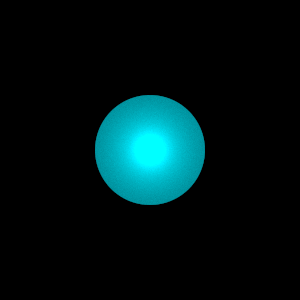
\includegraphics[scale=0.5]{SSL.png}
\caption{Simple Spot Light - light is emitted from 1 point uniformly in cone}
\end{figure}

Fading Spot Light is like Uniform Spot Light, but it is deliberately dimmer further from center of cone.
\begin{figure}[H]
\centering 
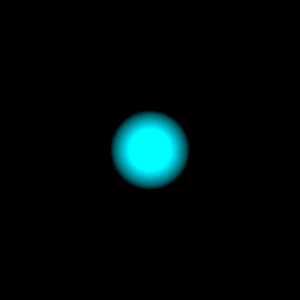
\includegraphics[scale=0.5]{FSL.png}
\caption{Fading Spot Light with slightly higher power}
\end{figure}
To do that, we can create sample set and turn it it into weighted random distribution. Spot light needs (besides position and direction) another parameter - cone angle, which is angle from direction in which beams can be generated. Fading spot light also needs parameter that describes fading. In this example, that parameter is \verb|fade_per_angle|, which describes how much percent dimmer should light shine. From \verb|cone_angle| and \verb|fade_per_adngle|, we can calculate \verb|fade_angle| as (\verb|cone_angle - 1/fade_per_angle|), which is an angle from which onward, light intensity is lowered by value of \verb|fade_per_angle|, per angle. Our Sample set would have $f(x) = 1$ for x from $[0,$\verb|fade_angle|$)$ and $f(x) = 1 - ($\verb|cone_angle| $- x)*$\verb|fade_per_angle| for other. Fading spot light class can look like this:
\begin{lstlisting}[language=Java]
public class  FadingSpotLight extends spdLightSource(){
  private Vector3 perpendicular;
  private WeightedRandomGenerator wrg; 
  private Random circlerot;
 	. . .

  public FadingSpotLight( . . .){
		. . .
	perpendicular = direction.getRandomCross();
	wrg = new WeightedRandomGenerator(. . .);
  }
 . . .
  public Beam getNextBeam(){
	Beam b = new Bean();
	b.lambda = spd.getNextLambda();
	b.origin = position;
	double angle = wrg.nextDouble();
	b.direction = direction.rotateTowards(
	  perpendicular, toRadians(angle));
	angle = circlerot.nextDouble()*360;
	b.direction = b.direction.rotateAround(
	  direction, toRadians(angle)); 
	number_of_beams++;
	return b;
  }
 . . .
}
\end{lstlisting}
\verb|WeightedRandomGenerator wrg| is our weighted random distribution for light intensity which is used to generate angle from [0, \verb|cone_angle|), with increasing bias against bigger angles. Spot light is simetrical on circles(around direction vector), so we can uniformly randomly turn new Beam.direction around spot light direction. This way, fading spot light has adjustable fade towards light cone edge.
 
\subsubsection{Simple "from-LightSource" rendering}
Process of simple rendering using \href{https://en.wikipedia.org/wiki/Diffuse_reflection}{Diffuse} material, and/or forced reflection/refraction and only 1 light source can be summarized as following:
\begin{enumerate}
\item Set up scene objects (Geometry and simple "material functions"), add Light source, add simple deterministic camera.
\item In cycle, call \verb|getNextBeam()|, check if it intersects with diffuse object, if yes: send that beam to camera from intersection point and generate new Beam. If no, and it intersect with nothing, generate new Beam, if it intersect with other than diffuse object, call its material function which will return new Beam. Check if this beam intersects with some scene object. Repeat till iteration limit per beam is reached. If this limit is reached, generate new beam.
\item After some iterations, let camera generate picture.
\end{enumerate}
Because of lacking material functions, this does not provide photorealism, but it is good enougth for some test picture.
\begin{figure}[H]
\centering 

\includegraphics[scale=0.4]{Reflection55.png}
\caption{Caustic only, on ring, low beam count}
\end{figure}
\begin{figure}[H]
\centering 
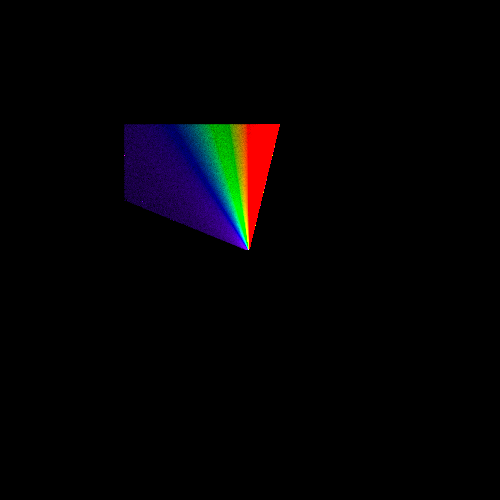
\includegraphics[scale=0.4]{Refraction117.png}
\caption{Top down, refraction of white light on prism}
\end{figure}
\begin{figure}[H]
\centering 
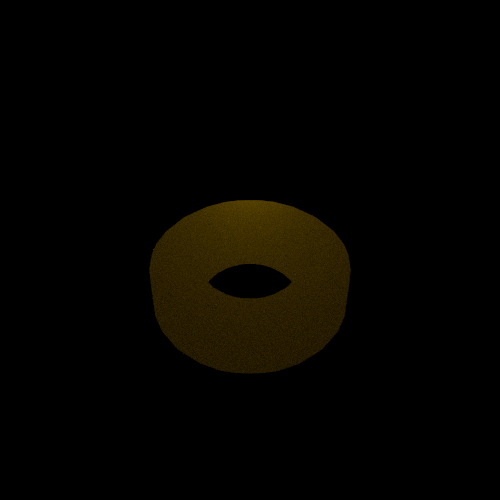
\includegraphics[scale=0.4]{Torus.png}
\caption{Diffuse torus, illuminated by SimpleSpotLight}
\end{figure}



%maybe do own section for all of Renderer subsections
\section{Renderer}
Next step is to create rendered using bidirectional path tracing, with SPD and Power as color representation which enables easy use of known light interaction rules and thus should result in easily created photo-like images.

\textbf{Following sections are stubs, they are subject to future development of this project}

\subsection{Scene}
Contains SceneObjects, Cameras (CameraManager) and lights 	(LightSourceManager), manages light/camera path tracing.
\subsection{Scene Objects}
Something that can interact with beams (light/camera). Provides ray 	intersection function, which returns new beam/LightSource using relevant material function. Scene should contain SceneObjectManager containing all SO.
\subsection{Camera}
Can create image from detected beam data, Can create camera beams, 	is aware of “master light source” - LightSourceManager
Scene should contain CameraManager, CameraManager contains all  	other sensors (Cameras)
\subsection{Light Sources}
% empty now
\subsection{Materials}
Have material function which takes beam and returns new Beam/LS.

\end{document}
